\documentclass[conference]{IEEEtran}
\usepackage[utf8]{inputenc}
\usepackage{fancyvrb}
\usepackage{cite}
\usepackage[pdftex]{graphicx}
\graphicspath{{./png/}}
\DeclareGraphicsExtensions{.png}
\usepackage[cmex10]{amsmath}
\interdisplaylinepenalty=2500
\usepackage[ruled,norelsize,linesnumbered]{algorithm2e}
%\usepackage{array}
\usepackage[para]{threeparttable}
\usepackage{multirow}
\usepackage{mdwmath}
\usepackage{mdwtab}
%\usepackage{eqparbox}
\usepackage[caption=false,font=footnotesize]{subfig}
\usepackage{fixltx2e}
%\usepackage{stfloats}
\usepackage{url}
\usepackage{tikz}
\usetikzlibrary{arrows,positioning} 

\makeatletter
\newcommand{\removelatexerror}{\let\@latex@error\@gobble}
\makeatother

\hyphenation{}

\begin{document}

% paper title
% can use linebreaks \\ within to get better formatting as desired
\title{Solving the Stereo Matching Problem Using an Embedded GPU for a Real-time Application}

\author{\IEEEauthorblockN{Pedro Aguiar\IEEEauthorrefmark{1},
Sébastien Varrier\IEEEauthorrefmark{4},
Jorge Lozoya\IEEEauthorrefmark{1},
Martha López\IEEEauthorrefmark{1} and
Damien Koenig\IEEEauthorrefmark{4}}


\IEEEauthorblockA{\IEEEauthorrefmark{1}Engineering Department\\
Universidad de Monterrey, San Pedro Garza García, Nuevo León 66238, México.\\
Email: \{pedro.aguiar, jorge.lozoya, martha.lopez\}@udem.edu}

\IEEEauthorblockA{\IEEEauthorrefmark{4}Laboratoire de Conception et d'Intégration des Systèmes\\
Grenoble INP / ESISAR, Valence 26902, France.\\
Email: \{sebastien.varrier, damien.koenig\}@esisar.grenoble-inp.fr}}

\maketitle

\begin{abstract}
General-purpose computing on graphics processing units (GPGPU) is used not only to offload the CPU from heavy computations but also to perform them faster than it is possible on CPUs. This is commonly referred as GPU acceleration and is an exercised area of study in the PC platform but has received very little attention when it comes to embedded devices. Just as the PC GPU is being used to perform computations that would otherwise be impossible in terms of execution time, the embedded GPU should be seen as a processor capable of accelerating computations with respect to its accompanying CPU. This effectively pushes the limits of what can be done with existing Systems on a Chip which have the advantage over the PC platform of being able to be used in portable devices. All the details of the implementation of a factible stereo matching real-time application for an embedded GPU are presented in this work. Details include the delimitation process, optimization techniques and even the source code.
\end{abstract}

% no keywords

\IEEEpeerreviewmaketitle

% - - - - - - - - - - - - - - - - - - - - - - - - - - - - - - - %

\section{Introduction}
This work presents new insight into the capabilities of using the embedded GPUs to perform computations having an engineering application.

The power restrictions that are inherited when designing a portable processor will always mean there is a stationary processor that can handle more computations in less time. Therefore problems attempted to be solved by a an embedded processor should not be the same problems that require significant computation power even for a stationary computer or, at the very least, a loss in accuracy or detail at the output should be expected. While you can not expect the same results from the embedded and the PC platform--this holds true for GPUs and CPUs--embedded GPUs have reached a point that is well worth of attention.

Portability opens a lot of possibilities and this is a feature that should be kept central when an embedded device is to be used. This work aims to highlight that while computation intensive problems (such as 3D reconstruction) can not be solved in real-time using current embedded GPU technology, the solveable tasks can be successfully applied even in time constrained applications. This makes currently available embedded GPUs a processing tool that should not be overlooked. We have the interfaces to the GPU and the processing power of some years ago with a degree of portability that was not possible then. Processing power is a common restriction on embedded environments that can be alleviated by putting the graphics processors to work.

This work consists of eight sections. In the first section some related work is presented for contextualization purposes. Second section introduces GPGPU and its limitations found in the embedded architecture. Next section shortly presents important theory and concepts of the graphics library of choice for a good understading of the work. Fourth section is about guidelines to get better time performance when using a GPU to perform computations and covers both CPU and GPU considerations. After that, the stereo matching problem is described and a case study is presented as the motivation and target of this research. Next section goes into detail about the design and implementation of the proposed solution including the chosen algorithm, used data structures, operations performed on them, key aspects of the GPU code and the description of a developed testing platform. Finally, results are discussed, conclusions are stated and possible further work is proposed.

% - - - - - - - - - - - - - - - - - - - - - - - - - - - - - - - %

\section{Related Work}
This work is mainly related to the stereo matching problem and using the graphics processing unit to accelerate computations to solve it. It is also narrowly related to performing GPGPU on embedded graphics processing units.

From the stereo matching point of view recent work has been published with new solution proposals. In \cite{bin05} a rectification-free binocular stereo vision which targets autonomous vehicles is presented. Also for moving vehicles, \cite{unger11} presents a method robust to inaccurately rectified images. Work has been done for eliminating the need of a maximum disparity and refinement of the result \cite{unger09}. Studies about modern \cite{olofsson10}, fast and robust \cite{hong10} algorithms to solve the stereo matching problem have been done recently, these include all kind of algorithms--including those that do not favor the GPU architecture. However, a study that is more related to the present work is that of \cite{jonsson03}, this study is aimed at implementing a fast, shader-based solution to the problem.

It is also of interest to this work that algorithms to solve this and other computer vision problems are usually explicitly flagged as highly parallelizable if it applies. Solutions with this characteristic will get performance boosts with recent (and upcoming) improved availability of parallel processing power resulting from multi-core CPU technologies and generalized interfaces to GPU processing. This is an important feature of algorithms that has been highlighted since decades \cite{baker81}.

On the GPU acceleration end, recent work has been done on multi-camera setups for real-time 3D reconstruction of faces \cite{denker11} and scenes \cite{woetzel04}. In \cite{zhao11} a faster-than-video method using multi-resolution adaptive windows is presented. However, all the previously mentioned work has been done on PC GPUs--on which research work is vast. Work on embedded platform can be found in \cite{singhal10} and \cite{singhal12}, where different computer vision algorithms (including stereo matching) were implemented using shaders and the results are evaluated. The work also presents techniques to achieve increased performance from shaders and discusses the embedded GPU in general. The interested reader can refer to \cite{singhal12} for more insight to the embedded GPU's evolution, key features and considerations.

A small field of interest--given the case study presented further in this document--to this work would be Raspberry Pi-based stereo systems. While computer vision is an area of interest amongst hobbyists, most of the few available work is conformed by either very simple and/or slow, CPU-and-OpenCV-based products. Only one formal publication about stereo vision on this platform was found by the authors \cite{neves13}. The work on this publication does not use the GPU and concludes 2-3 fps are attainable.

% - - - - - - - - - - - - - - - - - - - - - - - - - - - - - - - %

\section{GPGPU and Embedded GPU}
General-purpose computing on graphics processing units is employing a GPU to perform computations typically done in a CPU. The main task of GPUs is graphics and everything related to this processors (hardware, drivers, APIs) was designed to perform graphics-related computations. It is for this reason that--historically--using the processing power of a GPU required reformulating the problems in terms of graphics (primitives, textures, framebuffers, color channels, etcetera) and using an available graphics API to compute the desired output. The two major graphics APIs are Khronos' OpenGL and Microsoft's Direct3D. The development of GPU technology brought modern interfaces to their processing power that allows to use them as general, parallel processing units. These interfaces include Khronos' OpenCL and NVIDIA's CUDA and gave GPGPU researchers the opportunity to completely forget about graphics and solve their problems without that previously required reformulation. The former, graphics-reformulation method is now referred to as Legacy GPGPU while computations done through OpenCL/CUDA are now commonly referred to as GPGPU.

Performing a desired operation in any data as fast as possible is usually the target behavior--specially if few or no accuracy is sacrificed--but time can be specially critical if (a) the dataset is huge in size and/or (b) the output has to meet some tight deadlines (not to enhance user experience but because there are other systems relying on it). If the desired operations fit well into the GPU's single instruction, multiple data (SIMD) architecture GPGPU can hardware-accelerate these solutions. For the first case, huge datasets should be approached using a high end processing unit to prevent extra milliseconds to add up to hours or days. For the second case--which fits into the category of using the output of the computation as a part of a control system--the best solution depends on the embeddability required by the system.

Embedded GPUs may lag behind their full featured PC counterparts in terms of processing cores and speed but they have the obvious advantages in size, portability, power consumption and price. Architecture details and common/key features can be found in \cite{singhal12}. These graphical processing units are found in Systems on a Chip (SoC) present anywhere from consumer electronics such as smartphones, tablets, videogame consoles to more exposed scenarios such as development or evaluation boards.

Available APIs to embedded GPU processing power is an ongoing problem. While some of the highest profile devices now support a version of OpenCL and/or CUDA most of the readily available commercial options do not. Highest profile products have equally high prices which may or may not be worth it for the application at hand. That said, the vast majority of embedded GPUs still rely on reformulating target problems in terms of graphics and using OpenGL ES 2.0 to compute a hardware accelerated solution. This is arguably the most important difference between PC and embedded GPUs because it does not only impact performance but also the way problems have to be approached is changed entirely because of this limitation.

OpenGL ES (Open Graphics Library for Embedded Systems) is a subset of the OpenGL specification--this major version is aimed at PC graphic cards--which is made to suit the capabilities and requirements of an embedded GPU. The 2.0 version of the specification is mature and widely supported. Important upgrades that provide more flexibility to the usage of the GPU's processing capabilities have been introduced to newer versions (3.0 and 3.1) of the specification but these are also only supported by a few end devices. For this reason, further OpenGL discussion presented in this work is focused on the ES 2.0 specification.

% - - - - - - - - - - - - - - - - - - - - - - - - - - - - - - - %

\section{OpenGL ES 2.0}
A quick introduction to the concepts used further in this document is presented in this section. A considerable amount of the content of this section was extracted from the specification \cite{opengles2}, refer to it for a more in-depth explanation of the mentioned concepts.

\begin{figure}[!t]
	\centering
	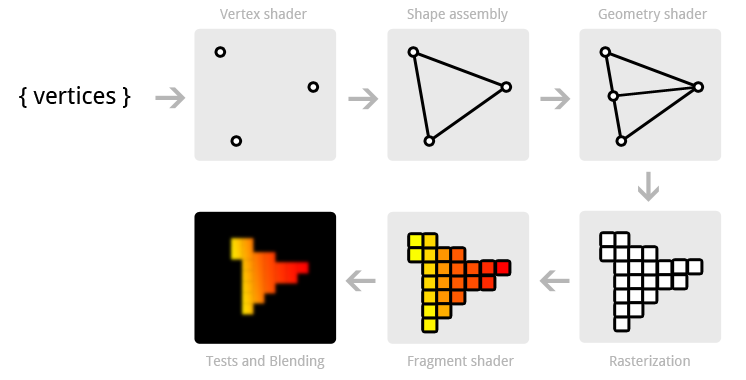
\includegraphics[width=3.0in]{shader_work}
	\caption{Results after each shader stage has been executed.}
	\label{fig:shader_work}
\end{figure}

	\subsection{OpenGL ES Shading Language}

		\subsubsection{Programs and shaders}
Body vertices are processed by the vertex shader. To use a vertex shader, shader source code is first loaded into a shader object and then compiled. Alternatively, pre-compiled shader binary code may be directly loaded into a shader object. In addition to vertex shaders, fragment shaders can be created, compiled, and linked into program objects. Fragment shaders affect the processing of pixel-sized fragments. A single program object must contain both a vertex and a fragment shader.

It is at the vertex shader where operations such as rotation, translation and scaling of bodies are performed. Fragment shaders set the color RGBA components of fragments of surfaces resulting from the vertices after they are processed by the vertex shader. Work done by each of these shaders is graphically shown in Figure \ref{fig:shader_work}.



		\subsubsection{Shader interactions}
Attributes variables are accessed by vertex shaders from an array of 4-component generic vertex attributes. They are meant to store attributes such as the coordinates and color of a vertex.

Uniforms are per-program variables that are constant during program execution. They retain their values once loaded, and their values are restored whenever a program object is used, as long as the program object has not been re-linked. Samplers are a special form of uniform used for texturing.

Varying variables hold the results of vertex shader execution that are used later in the pipeline. A vertex shader may define one or more varying variables. These values are expected to be interpolated across the primitive being rendered.

Interactions between the previously mentioned types of variables are shown in Figure \ref{fig:shader_interaction}. It is shown that uniforms can be read from both shaders, but the other types of variables flow from attributes passed into the vertex shader to the output of the fragment shader.

\begin{figure}[!t]
\centering
	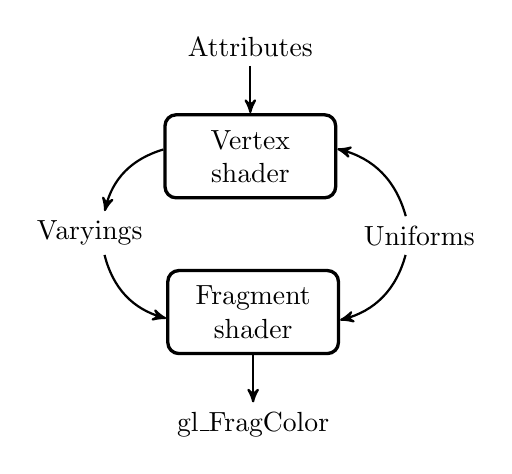
\begin{tikzpicture}[node distance=0.6cm, auto, >=stealth', nodestyle/.style={ rectangle, rounded corners, draw=black, very thick, text width=5.5em, minimum height=3em, text centered}, pil/.style={->, thick}]
	 \node (sout) {gl\_FragColor};
	 \node[nodestyle, above=of sout] (fs) {Fragment shader};
	 \node[above right=0.25cm of fs] (uni) {Uniforms};
	 \node[above left=0.25cm of fs] (var) {Varyings};
	 \node[nodestyle, above left=0.3cm of uni] (vs) {Vertex shader};
	 \node[above=of vs] (attr) {Attributes};
	 \path
	  (attr) edge[pil] node [below] {} (vs)
	  (vs) edge[pil, bend right] node [left] {} (var)
	  (var) edge[pil, bend right] node [below] {} (fs)
	  (uni) edge[pil, bend right] node [above] {} (vs)
	  (uni) edge[pil, bend left] node [below] {} (fs)
	  (fs) edge[pil] node [below] {} (sout);
	\end{tikzpicture}
	\caption{Diagram of the interactions between shaders to compute the color of a fragment and the involved variables in the process}
	\label{fig:shader_interaction}
\end{figure}

	\subsection{Texturing and Framebuffers}
		\subsubsection{Textures}
Classical use of textures is to apply color to bodies and these are typically loaded by the CPU from image files but they can also drawn by the GPU. Texture lookups map a portion of one or more specified images onto a fragment or vertex. This mapping is accomplished in shaders by sampling the color of an image at the location indicated by specified texture coordinates.

		\subsubsection{Framebuffers}
OpenGL ES writes to (and reads values from) a framebuffer. Framebuffers can be window-system-provided (which would be the device screen or some area of it) or application created framebuffers (which are used to write to textures after they are bound together and would not directly reflect on the device screen).

		\subsubsection{Formats}
Two formats are mentioned further in this work: LUMINANCE and RGBA. LUMINANCE format means only grayscale data is present and RGBA means red, green, blue and alpha components are present. Framebuffers must have R, G, B, and, optionally, A unsigned integer values. Therefore, LUMINANCE data must be expanded to RGB or RGBA data if a framebuffer will be bound to it.

		\subsubsection{Minification and magnification}
Mignification is when a texture is drawn onto a smaller surface and magnification is when a texture is drawn onto a larger surface.

		\subsubsection{Mipmap}
an ordered set of arrays representing the same image; each array has a resolution lower than the previous one. The source image is the level zero array and must have power of two dimensions for both width and height. Each array subsequent to the level zero array has half the dimension of the previous level on each direction (if the dimension in any direction of the previous level is one the dimension in the given direction remains one), until the last array is reached with dimensions one by one. A graphical explanation is shown in Figure \ref{fig:mipmap_explanation}.

\begin{figure}[!t]
	\centering
	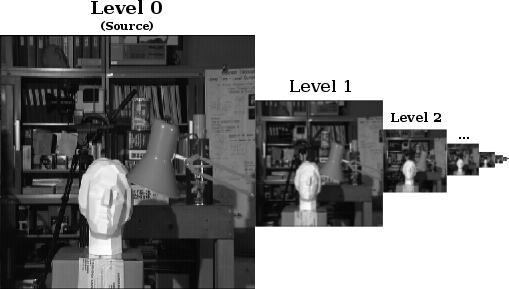
\includegraphics[width=3.0in]{mipmap_explanation}
	\caption{Mipmap array of the Tsukuba left image}
	\label{fig:mipmap_explanation}
\end{figure}

	\subsection{Web Graphics Library}
WebGL is another graphics API from the Khronos Group that is supported by major web browsers in both PC and mobile platforms. WebGL is described as ``OpenGL ES 2.0 for the Web" by Khronos because of their vast similarities. Shaders written for WebGL work without any modifications on OpenGL ES 2.0. Other GPU setup operations such as buffers, textures and framebuffers creation, deletion and binding are exactly the same. This similarity between APIs was exploited in this work to benchmark the proposed algorithm running on different embedded GPUs through WebGL.

% - - - - - - - - - - - - - - - - - - - - - - - - - - - - - - - %

\section{GPU Coding for Performance}
Performance when programming for a GPU is not only a function of the written code but also of the underlying hardware--and the software between them (operating system, drivers). The fastest out of two approaches of solving a computational problem can vary depending on these factors. An example for this is that data transfers between the CPU and the GPU are historically believed to be a bottleneck in terms of performance and different CPU/GPU workarounds can be implemented--data compression, packing or breaking. Running the same code in Unified Memory Architecture implementations (both processors share the pool of memory, removing the data transfers problem) may dim all the introduced workarounds as the new--unnecessary--bottleneck. Absolutely best performance is often achieved by custom solutions for the target hardware/software combination. That said, there are some things to have in mind when writing code involving the GPU which almost certainly hold true across the different combinations of hardware and software and these are presented in this section.

	\subsection{GLSL guidelines}
Here is a short list of programming tips for OpenGL ES 2.0 shaders. The following programming tips are found in \cite{singhal12} and \cite{appleopengl}. The interested reader should refer to these sources for a more detailed explanation.

\begin{itemize}
\item \emph{Precision control.} Using more precision than required adds up execution time. Adjust the precision to the lowest value that works. Precision ranges can be hardware dependent.
\item \emph{Branching.} Having multiple branchless shaders may be faster than a single branched one. If a branch can not be avoided it is best to branch on constants, then uniforms and, lastly, a computed value.
\item \emph{Loop unrolling.} Make sure you can not avoid using a loop by using vectors. If that is not possible unrolling the loop by hand may produce better performance. Constant loop limits are preferred due to branching.
\item \emph{Arrays.} Using indices computed in the shader is more expensive than a constant or uniform array index. Accessing uniform arrays is usually cheaper than accessing temporary arrays.
\item \emph{Use varying interpolators.} If a value linearly changes with a varying variable it is better to use another varying variable to compute it. The most common example is to calculate the coordinates of the pixels around the current pixel to avoid a dependent read.
\item \emph{Perform vector calculations lazily.} For example, if you are multiplying two sacalars and a vector it is important that you arrange the code so the scalars are multiplied first and the result of this operations is multiplied by the vector. This may increase performance if the graphics processor does not have a vector processor.
\end{itemize}

	\subsection{OpenGL guidelines}
Shaders are run by the GPU but the GPU is still a CPU peripheral. If the CPU code controlling the graphics processor is poorly written then performance will be affected. Here are some guidelines to keep in mind when writting the code that commands the GPU.

\begin{itemize}
\item \emph{Texture compression.} OpenGL ES supports texture compression. If you application is not affected by a small loss of quality, using texture compression can boost performance.
\item \emph{Fewer state changes.} Minimize OpenGL state changes. Switching textures, programs, buffers, etcetera must only be done if necessary.
\item \emph{Fewer syncing and getter functions.} If you make a function call from the GPU that syncs it with the GPU that will be very slow. Examples of these functions are \texttt{readPixels()} and \texttt{finish()}. Also getter functions such as \texttt{getUniformLocation()} should be avoided by caching the results whenever it is possible.
\item \emph{Mipmaps.} GPUs usually have accelerated ways to compute the mipmap of a texture. A read from a mipmap-complete texture is automatically done at a convenient lower level of detail and this increases performance.
\item \emph{Texture packing}. When working with LUMINANCE textures you may end up wasting three data channels. When using this format you get a texture where $R=G=B=I$ and $A=1.0$ but it is possible to use these unused channels to store other texture or any other data. For example, given the 4x4 LUMINANCE texture
\begin{equation*}
\label{eq:luminance}
\begin{bmatrix}
I_{1,1} & I_{1,2} & I_{1,2} & I_{1,3}\\ 
I_{2,1} & I_{2,2} & I_{2,2} & I_{2,3}\\ 
I_{3,1} & I_{3,2} & I_{3,2} & I_{3,3}\\ 
I_{4,1} & I_{4,2} & I_{4,2} & I_{4,3}
\end{bmatrix}
\end{equation*}
the RGBA representation of the first column would be (notice the repeated data)
\begin{equation*}
\label{eq:rgba}
\begin{bmatrix}
\{I_{1,1}, I_{1,1}, I_{1,1}, 1.0\}\\ 
\{I_{2,1}, I_{2,1}, I_{2,1}, 1.0\}\\ 
\{I_{3,1}, I_{3,1}, I_{3,1}, 1.0\}\\ 
\{I_{4,1}, I_{4,1}, I_{4,1}, 1.0\}\\ 
\end{bmatrix}
\end{equation*}
The four LUMINANCE columns can be losslessly packed into a single RGBA column. Resulting in 
\begin{equation*}
\label{eq:rgbapacked}
\begin{bmatrix}
\{I_{1,1}, I_{1,2}, I_{1,3}, I_{1,4}\}\\ 
\{I_{2,1}, I_{2,2}, I_{2,3}, I_{2,4}\}\\ 
\{I_{3,1}, I_{3,2}, I_{3,3}, I_{3,4}\}\\ 
\{I_{4,1}, I_{4,2}, I_{4,3}, I_{4,4}\}\\ 
\end{bmatrix}
\end{equation*}

Graphical results of doing this horizontally and vertically are shown in Figure \ref{fig:hor_ver_packing}. Another option is to pack four textures into one. Analysis is similar and the output can be seen in Figure \ref{fig:gray2color_packing}.
\end{itemize}

\begin{figure}[!t]
	\centering
	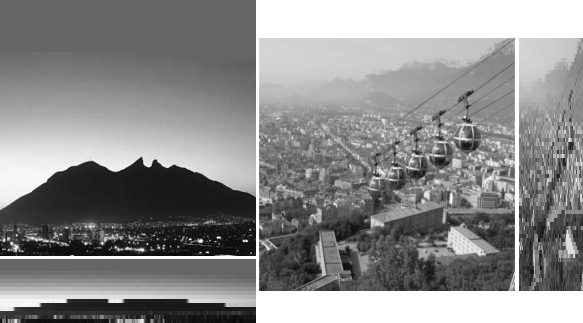
\includegraphics[width=3.0in]{hor_ver_packing}
	\caption{Horizontal and vertical packing of grayscale images}
	\label{fig:hor_ver_packing}
\end{figure}

\begin{figure}[!t]
	\centering
	
\includegraphics[width=2.0in]{gray2color_packing}
	\caption{Packing four LUMINANCE textures into the color channels of a RGBA texture}
	\label{fig:gray2color_packing}
\end{figure}

% - - - - - - - - - - - - - - - - - - - - - - - - - - - - - - - %

\section{Stereo Matching and Case Study}
Stereo matching consists in matching a point found in an image with its corresponding point(s) in other image(s). The importance of this information relies in the basic concept that if the displacement of a given point from one image to another and the parameters of each camera are known the depth of the point can be calculated. This can be well understood by using our eyes as an example. If you hold an object 10cm apart from your eyes and see it with your left and right eyes alternatively it will be displaced a longer distance than an object that is 2m appart. Higher disparity means closer object. This can be graphically seen in Figure \ref{fig:stereo_setup}.

\begin{figure}[!t]
	\centering
	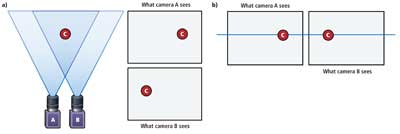
\includegraphics[width=3.0in]{stereo_setup}
	\caption{Stereo cameras setup and the disparity of a point}
	\label{fig:stereo_setup}
\end{figure}

When you search for a corresponding point in the other image similarity is measured, different quantities have been proposed to measure similarity. Refer to \cite{hong10} for some commonly used robust similarity quantities. It is also a common practice to not only measure the similarity of a point but also the similarity of its surroinding pixels, this is commonly referred to as a support window and is done to reduce false-positives since two neighbor pixels can be very similar--or even exactly the same. This is shown in Figure \ref{fig:support_windows}. Also shown is that search is commonly done through a single row of the image if both images of a binocular systems are set up (or the resulting images are rectified) so height is the same in both images. This is a special case for the epipolar geometry when the image planes coincide and can reduce the search significantly.

\begin{figure}[!t]
	\centering
	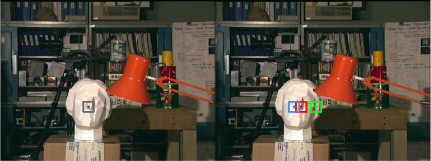
\includegraphics[width=3.0in]{support_windows}
	\caption{Support windows, pixel and its window to be matched on the left and attempted windows on the right}
	\label{fig:support_windows}
\end{figure}

Once the disparity of each of the matched pixels in an image is computed that image's disparity map is known. The disparity equation 

\begin{equation}
\label{eq:disparity}
d = \frac{Bf}{Z}
\end{equation}

can be applied to solve for the depth of the corresponding body. $B$ is the baseline, $f$ is the focal length and $Z$ is the depth.

The initial motivation of researching the current capabilities of the embedded GPU was to use it to solve the stereo matching problem to detect and calculate the distance to the next object ahead of an autonomous vehicle instrumented with a simple left-right binocular system. Therefore, the implemented solution is aimed at this particular case.

The mentioned case study allows for certain relaxation that was used to fit a faster solution into the GPU. Important points are:

\begin{itemize}
	\item \emph{Only the distance to the next object is required:} the data sent back to the CPU can be packed into a single pixel. Four pixels are sent back to the CPU in the implemented solution. The pixels correspond to the distance to the closest object at each fourth part of the image.
	\item \emph{Very small objects can be flagged as irrelevant:} the required density of the computation is not high. This was used to filter small, wrongly-matched areas from the image.
	\item \emph{Objects ahead in the vehicle's lane are expected to be centered:} the search can be limited to a region of interest (Fig.~\ref{fig:highway_camera}). Only a centered $256\times256$ pixels area is matched in this work.
	\item \emph{Left-right binocular system:} an object in the left image can only be dispaired to the left on the right image.
\end{itemize}

\begin{figure}[!t]
	\centering
	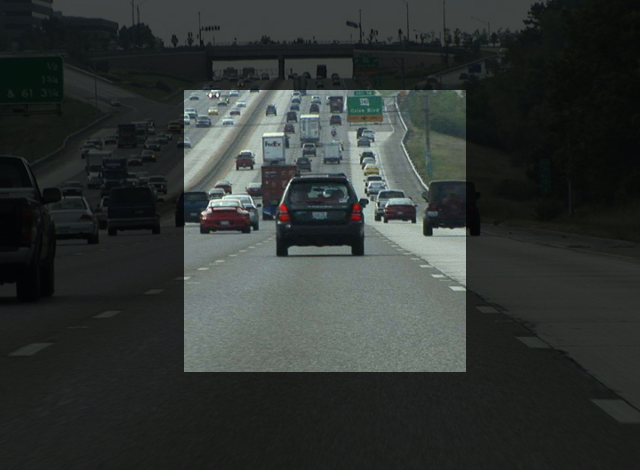
\includegraphics[width=3.0in]{highway_camera}
	\caption{Camera in the front of a vehicle. Most of the image does not carry information about the object ahead}
	\label{fig:highway_camera}
\end{figure}

% - - - - - - - - - - - - - - - - - - - - - - - - - - - - - - - %

\section{OpenGL ES 2.0 Based Implementation}
This section describes in detail the design decisions taken to perform the stereo matching using an embedded GPU. The implementation aims for performance so it uses a local method which matches and takes advantage of functionality exposed by the OpenGL ES 2.0 API. The matching algorithm is not described in full detail and discussion is oriented towards the OpenGL features. Refer to \cite{jonsson03} for details on why a local, hierarchical algorithm matches the GPU architecture and for a detailed description of a similar algorithm. Alternatively, source code is availbale for the current implementation in \cite{aguiar14} and can be used to understand in full detail.

	\subsection{Hierarchical algorithms using OpenGL mipmaps}
A hierarchical method is used to generate the disparity map. The principle behind these methods is calculating the disparity map at a low resolution and then use it as the input for the next level of detail. This approach is very convenient for an OpenGL ES 2.0 implementation because its concept of mipmap can be used to closely match this hierarchical principle with three major benefits: (1) better performance due to GPU reading the texture of the most convenient size, (2) mipmaps are very important in graphics-intensive software and therefore this operation is usually natively very fast for GPUs and (3) setting an interpolating minification filter results in each outputted pixel holding information about their surrounding pixels (which is what support windows are used for). The impact of using an interpolating minification filter is shown in Figure \ref{fig:filters}. The non-interpolating filter is \texttt{GL\_NEAREST} which simply outputs closest pixel in coordinates from the source texture. The interpolating filter is \texttt{GL\_LINEAR\_MIPMAP\_NEAREST} which performs a bilinear filter when calculating the lower levels of detail of a texture.

Mipmaps and interpolating filters are key OpenGL ES 2.0 features for the fast implementation presented in this work. If mipmaps were not used then lower levels of detail for the source images and their respective support windows must had been computed by iteratively convolving using downsampling and blurring kernels. This would require more memory (programs, textures and framebuffers), state changes (changing active program, textures, framebuffer, updating uniforms) and rendering stages which would result in longer execution time and increased complexity. OpenGL ES 2.0 specification states that mipmaps can only be generated for textures whose both width and height dimensions are powers of two (POT) and this is the most important reason to only compute the disparity map of a region of $256 \times 256$ pixels. If the application requires to compute bigger areas it can be done as long as both dimensions are still a powers of two ($512 \times 256$ or $512 \times 512$). A camera that can output on different, configurable resolutions is desired to set up working, convenient parameters.

\begin{figure}[!t]
	\centering
	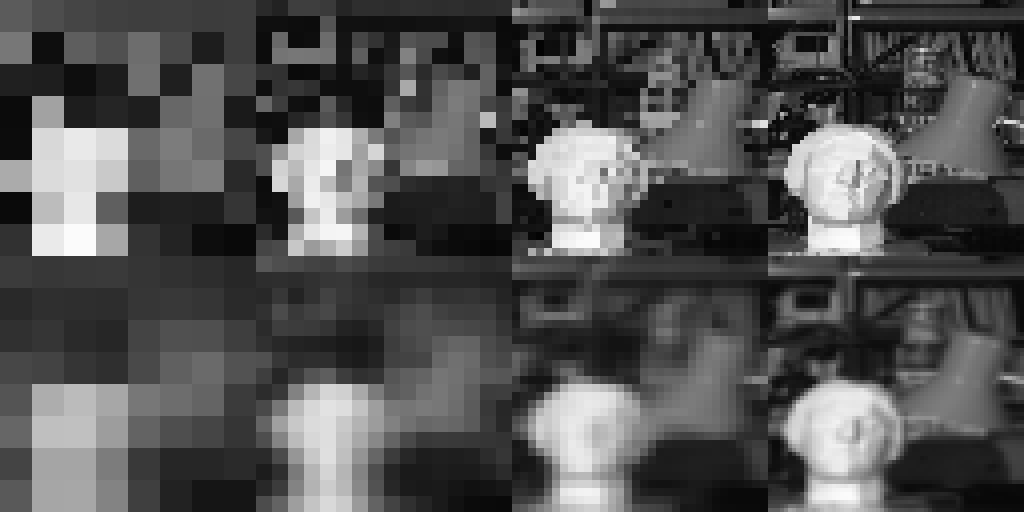
\includegraphics[width=3.0in]{filters}
	\caption{Same section of the Tsukuba left image drawn with different levels of detail using a non-interpolating minification filter (above) and an interpolating one (below)}
	\label{fig:filters}
\end{figure}

	\subsection{CPU side}
The GPU performs computations it is commanded to by the CPU. There is GPU-related code that is executed in the CPU and impacts GPU performance. This code includes OpenGL and EGL setup to get an area of the screen to draw onto, initialization tasks such as texture and framebuffer creation or program compilation and linkage, state changes occurring at each drawing iteration such as changing the active texture, framebuffer or program, setting attributes/uniforms and other data transfers such as writing a texture or reading a framebuffer.

To achieve the best GPU performance CPU code modularization has to be reduced. Coming from a CPU-programming background it may be tempting to write a \texttt{runShader()} function that takes the used shader, textures and target framebuffer as well as some values to be assigned to its uniforms as arguments. While this will result in shorter and cleaner CPU code it impacts GPU performance due to unnecessary queries to the GPU (requesting the uniform locations) and redundant state changes requests produced by binding a texture or framebuffer that was already bound or activating a program that was already active. To avoid these performance penalties the calls to OpenGL functions were minimized during the drawing loop by taking the modularization penalty and caching uniform locations. Also, all the actions that could be done only once were moved out of the drawing loop to an initialization function. The initialization steps are shown in Figure \ref{fig:alg:init}. Properties of textures mentioned in this algorithm are shown in Table \ref{tab:texturesprop}.

\begin{figure}[!t]
\removelatexerror
\begin{algorithm}[H]
\caption{Initialization}
	Set up OpenGL and EGL\;
	\For( \emph{(For each program)}){$p := 1$ to $P_{N}$}
	{
		Compile and link shaders\;
		Bind buffer with the vertices of a square\;
		Set uniforms that do not change during runtime\;
		Save locations of changing uniforms\;
	}
	Create textures, bind framebuffers\;
	Bind common textures to an active slot\;
\end{algorithm}
\caption{Setup and initialization on the CPU side}
\label{fig:alg:init}
\end{figure}

\begin{table}
\renewcommand{\arraystretch}{1.3}
\centering
\begin{threeparttable}
\caption{Used textures and their properties}
\label{tab:texturesprop}
\begin{tabular}{|c|c|c|c|c|}
\hline
\bfseries No. & \bfseries Holds & \bfseries Width & \bfseries Height & \bfseries Format\\
\hline
1 & Input Left & * & * & \multirow{2}{*}{LUMINANCE}\\\cline{2-4}
2 & Input Right & * & * & \\
\cline{2-5}
3 & Region of interest & 256 & 256 & \multirow{9}{*}{RGBA}\\ \cline{2-4}
4 & \multirow{5}{*}{Disparity maps} & 16 & 16 & \\\cline{3-4}
5 & & 32 & 32 & \\\cline{3-4}
6 & & 64 & 64 & \\\cline{3-4}
7 & & 128 & 128 & \\\cline{3-4}
8 & & 256 & 256 & \\\cline{2-4}
9 & \multirow{3}{*}{\begin{tabular}[x]{@{}c@{}}Filtering and\\maximum search\end{tabular}} & 16 & 16 & \\\cline{3-4}
10 & & 16 & 2 & \\\cline{3-4}
11 & & 2 & 2 & \\
\hline
\end{tabular}
\begin{tablenotes}
\item [*] These dimensions can be any size and depend on the resolution of the camera
\end{tablenotes}
\end{threeparttable}
\end{table}

Besides initialization operations the CPU still has to command actions such as setting the active progam, binding textures and framebuffers, setting the viewport, drawing and mipmap generation. The objective of the specific tasks commanded by the CPU for this implementation and the involved textures at each of these steps are shown in Figure \ref{fig:alg:loop}. Step 1 packs a region of interest ($256 \times 256$) for both left and input images into the red and green channels of Texture 3. This step allows to generate the mipmaps by getting a POT texture but also--due to the channel packing--the mipmaps of both textures are calculated with a single call to \texttt{glGenerateMipmap()} (Step 2). The next step (Step 3) attempts the matching at low resolution for only a pair of disparity values (0 and 1). The loop from Step 4 to Step 7 doubles the resolution of the previous disparity map, doubles the disparity value and then averages it with the surrounding pixels convoluting using a $3\times 3$ blurring kernel (Step 5). The next stereo matching attempt uses the available disparity as an input value and computes the best value from the neighbor pixels (Step 6). When the loop finishes a $256 \times 256$ disparity map has been computed.

\begin{figure}[!t]
\removelatexerror
\begin{algorithm}[H]
\caption{OGL ES 2.0 stereo matching}
	Crop and pack into RG channels : $(T_1, T_2)\rightarrow T_3$\;
	Generate mipmaps : $T_3$\;
	Lowest resolution ($16\times16$) matching : $T_3 \rightarrow T_4$\;
	\For(){$i := 5$ to $8$}
	{
		Double the resolution : $T_{i-1} \rightarrow T_i $\;
		Stereo matching with initial values : $(T_3, T_{i}) \rightarrow T_i$\;
	}
	Downsampling with dilate filter : $T_8 \rightarrow T_9$\;
	Search the maximum horizontally : $T_9 \rightarrow T_{10}$\;
	Search the maximum vertically : $T_{10} \rightarrow T_{11}$\;
\end{algorithm}
\caption{Algorithm of hierarchical stereo matching using OpenGL ES 2.0 and the involved textures (texture numbering is that of Table \ref{tab:texturesprop})}
\label{fig:alg:loop}
\end{figure}

The implemented hierarchical method is very fast because of its simplicity and the lack of any technique to smooth the output. The resulting disparity map holds the correct disparity of the foreground objects but it also includes noise at these areas and very noticeable errors at the background and occluded areas. The next step (Step 8) uses two assumptions of the given case study: (1) very small objects are irrelevant and (2) the distance to the closest object ahead is needed. The implemented filter downsamples the disparity map to a $16 \times 16$ texture and sets every pixel to the minimum of four tested pixels (dilate filter). This results in small objects being filtered to a small value while bigger objects still appear on the outputted map. Small values will not interfere when searching for the closest object (maximum value). Different case studies can use other filtering techniques depending on the assumptions that can be made of them. Finally, Step 9 and Step 10 draws the maximum value out of eight pixels into a single one horizontally and vertically, respectively. The result is a $2 \times 2$ texture holding the disparity of the closest object for each fourth part of the image. A diagram showing these stages and the involved textures is shown in Figure \ref{fig:pipeline}. The final state of textures three to eleven is shown in Figure \ref{fig:texturesfinal}.

\begin{figure*}[!t]
\centering
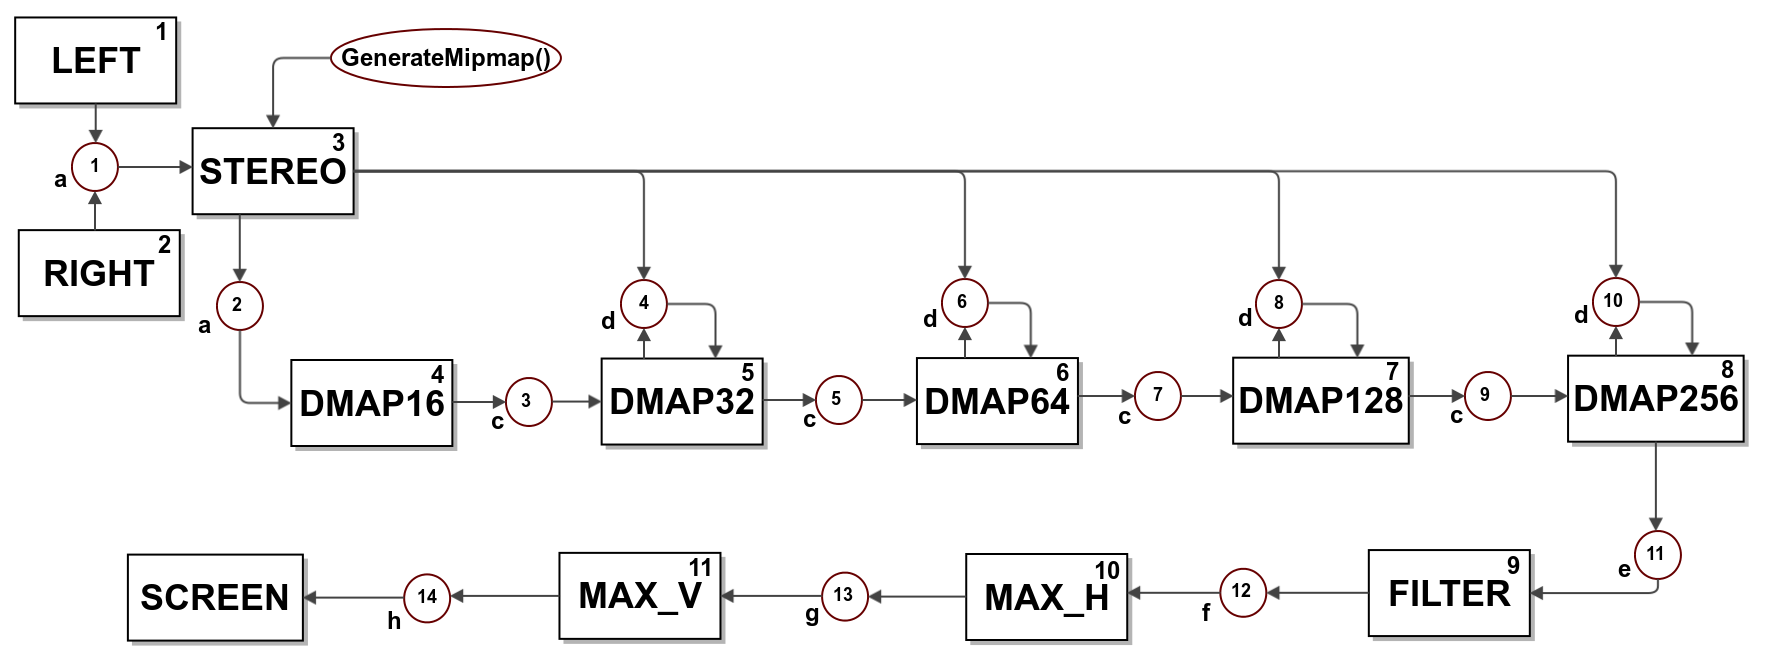
\includegraphics[height=1.8in, width=6.5in]{pipeline}
\caption{Rendering pipeline}
\label{fig:pipeline}
\end{figure*}

\begin{figure}[!t]
	\centering
	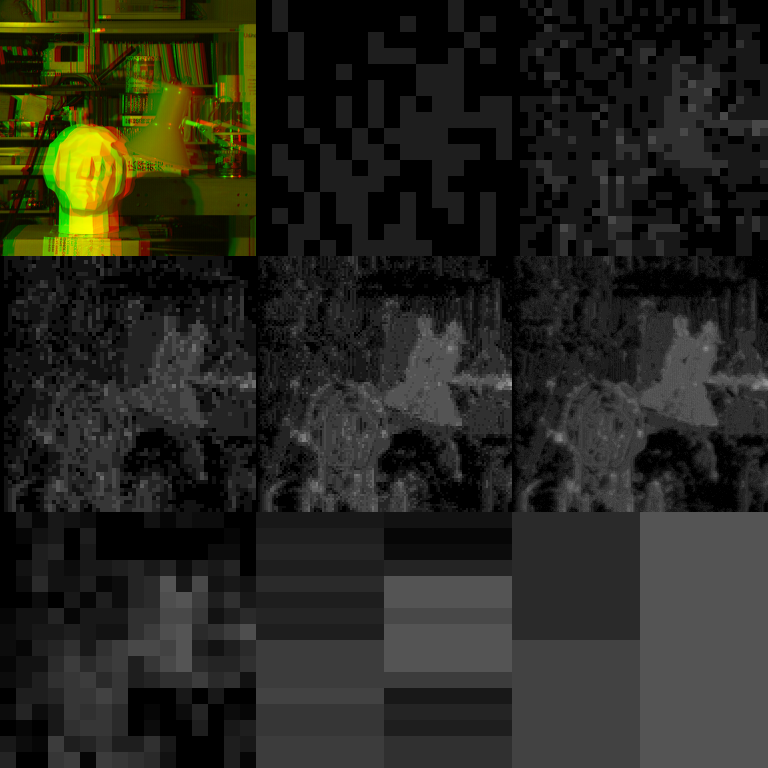
\includegraphics[width=3.0in]{texturesfinal}
	\caption{Final state of textures three to eleven after the matching algorithm has been performed (contrast of disparity maps was increased for visualization purposes)}
	\label{fig:texturesfinal}
\end{figure}

	\subsection{The shaders}
The operations of the steps shown in the algorithm of Figure \ref{fig:alg:loop} are performed in the GPU. As mentioned earlier in this document, a pair of shaders (vertex and fragment) form a program. The presented implementation uses ten programs made from mixing seven vertex shaders and seven fragment shaders.

All the vertex shaders perform scaling and offsetting of the vertices coordinates. These are always used to draw a centered square. The main difference between vertex shaders is the number of texture coordinates they set and the assigned value to them:
\begin{itemize}
	\item {\bfseries Simple.} Sets a varying for the texture coordinate at the current position.
	\item {\bfseries Flip.} Same as simple but flips the Y axis. Used for the final drawing.
	\item {\bfseries Crop.} Scales the texture coordinates to capture a region of the texture.
	\item {\bfseries Diagonals.} Sets a varying for each of the four diagonal directions from the current position.
	\item {\bfseries Interpolate.} Diagonals and current position are set.
	\item {\bfseries Line8.} Sets varyings for a line of eight texture coordinates.
	\item {\bfseries Left.} Sets two varyings, one for the current position and one for the left pixel. The code for this shader is shown in Figure \ref{fig:vs_left}. The code for the rest of the shaders can be found at \cite{paguiar14}.
\end{itemize}

\begin{figure}[!t]
	\begin{Verbatim}[frame=single,fontsize=\scriptsize]
precision lowp float;
uniform vec2 texelsize;
uniform vec2 offset;
uniform vec2 scale;
attribute vec4 vertex;
varying vec2 tc;
varying vec2 tc_l;

void main(void) 
{
	vec4 pos = vertex;
	tc = pos.xy;
	tc_l = tc + vec2(-1.0, 0.0) * texelsize;
	pos.xy = pos.xy * scale + offset;
	gl_Position = pos;
}
	\end{Verbatim}
	\caption{Left vertex shader source code}
	\label{fig:vs_left}
\end{figure}

Fragment shaders, when referring to output in the next list it is a reference to the gl\_FragColor value.
\begin{itemize}
	\item {\bfseries Channelpack.} Samples to textures and outputs them to R and G channel, respectively.
	\item {\bfseries Dmap0.} Sets the output to the disparity (0 or 1) that gets the most similar results.
	\item {\bfseries Dinterpolate.} Doubles an approximation of the average value of a pixel and its eight neighbor pixels.
	\item {\bfseries Dilate.} Sets the output color to the  minimum of four sampled pixels from the same texture.
	\item {\bfseries Erode.} Sets the output color to the maximum of eight sampled pixels from the same texture.
	\item {\bfseries Simple.} Sets the output to the sampled pixel from a texture.
	\item {\bfseries DmapN.} Reads a texture and samples three pixels from another texture depending on the read value. Sets the output to the disparity that gets the most similar results. Code of this shader is shown in Figure \ref{fig:fs_dmapN}. Note how branching is avoided using the \texttt{min()} function by previously multiplying the similarity and then packing the disparity at the fractional part. This achieves very fast performance.
\end{itemize}

	\subsection{WebGL platform and WebGL stats}
Given the lack of tools to work with the GPU, a WebGL platform was set up. This has very convenient advantages to support debugging, profiling and documentation (output can be saved as images). Also, since WebGL is a javascript API it has no compilation time and the APIs are similar enough that the resulting code can be easily translated to the preferred language of the target embedded platform.

The existence of WebGL also allows to test the results on different devices. Any embedded device with a WebGL-compatible set up can run the same code to compare performance. Results may vary across devices because the OpenGL specification is not very strict.

Another source of variation is the device capabilities. There are a number of constants that modify the bevavior. As of September 2014 the stats shown in \cite{singhal12} are not very restrictive and show positive tendencies. Some important constants are:
\begin{itemize}
\item \emph{MAX\_VARYING\_VECTORS.} The maximum number four-element floating-point vectors available for interpolating varying variables used by vertex and fragment shaders. Coverage includes 8 (99.2\%), 10 (75.3\%), 14 (59.0\%), 15 (59.0\%), 16 (55.3\%), 28 (0.2\%) and 31 (0.2\%).

\item \emph{MAX\_VERTEX\_UNIFORM\_VECTORS.} The maximum number of four-element floating-point, integer, or boolean vectors that can be held in uniform variable storage for a vertex shader. Coverage includes 64 (100\%), 128 (100\%), 250 (90.7\%), 512 (1.7\%), 768 (1.3\%) and 1024 (1.3\%).

\item \emph{MAX\_COMBINED\_TEXTURE\_IMAGEUNITS.} The maximum supported texture image units that can be used to access texture maps from the vertex shader and the fragment processor combined. Coverage includes 8 (100\%), 16 (72\%), 20 (68.7\%) and 32 (56.7\%).

\item \emph{MAX\_TEXTURE\_SIZE.} The value gives a rough estimate of the largest texture that the GL can handle. Coverage includes 1024 (100\%), 2048 (100\%), 4096 (92.2\%), 8192 (3.6\%) and 16384 (0.4\%).
\end{itemize}

\begin{figure}[!t]
	\begin{Verbatim}[frame=single,fontsize=\scriptsize]
precision lowp float;
uniform sampler2D stereo;
uniform sampler2D dmap;
uniform vec2 texel;
varying vec2 tc;

void main(void)
{
 float match = texture2D(stereo, tc).r;
 float dfloat = texture2D(dmap, tc).r;
 mediump float d = dfloat * 255.0;

 vec3 candidates = vec3(
  texture2D(stereo, tc - vec2((d - 1.0)*texel.x, 0.0)).g,
  texture2D(stereo, tc - vec2(d * texel.x, 0.0)).g,
  texture2D(stereo, tc - vec2((d + 1.0)*texel.x, 0.0)).g
 );

 mediump vec3 sim = ceil(abs(match - candidates) * 150.0);
 sim.g += 0.0039;
 sim.b += 0.0078;

 gl_FragColor = vec4(
  dfloat + fract(min(min(sim.r, sim.g), sim.b)) - 0.0039,
  0.0, 0.0, 1.0
 );
}
	\end{Verbatim}
	\caption{DmapN fragment shader source code}
	\label{fig:fs_dmapN}
\end{figure}




% - - - - - - - - - - - - - - - - - - - - - - - - - - - - - - - %

\section{Results and discussion}



% - - - - - - - - - - - - - - - - - - - - - - - - - - - - - - - %

\section{Conclusion and Further Work}

A highly optimized for fast performance solution to a case study involving the stereo problem was presented. Performance was achieved by GPU accelerating the computation of the disparity map, carefully selecting the OpenGL ES 2.0 functionality to be used and keeping every algorithm operation close to the available graphics functionality. The resulting disparity map is not perfect but holds useful information which can be filtered and sent back to the embedded CPU. While it is known and has been proved in other work that an embedded GPU can outperform its CPU counterpart, this work focused on calculating a fast approximation and filtering the results to get the required data at frequencies applicable to engineering problems with tight time constrains. Results section provides evidence that the embedded GPU is a processing power source that is already capable of pushing SoC processing limits further by computing solutions very fast if the required computations match the single instruction, multiple data architecture. If this condition is met the GPU could provide streaming, real-time operation for signal analysis.

Modern embedded GPU interfaces such as OpenGL ES 3.0, CUDA and OpenCL will be more adopted as more new, capable hardware reaches the market and the newly exposed functionality will open more embedded GPGPU applications, closing the gap between this and the PC platform--which will always be faster but also less portable. It is up to engineers to put this embedded processing power to use to develop solutions where the current embedded CPU is not the right processing unit in the chip.

%\IEEEtriggeratref{8}
%\IEEEtriggercmd{\enlargethispage{-5in}}

\bibliographystyle{IEEEtran}

\bibliography{IEEEabrv,ieeeconf.bib}

\end{document}
